\chapter{Périmètre, aire et volume}\label{ChPerimetresAires}

\begin{acquis}
\begin{itemize}
\item réaliser des conversions d'unités de longueurs;
\item réaliser des conversions d'unités d'aires;
\item calculer à partir d'une formule, l'aire d'un triangle, d'un carré, d'un rectangle, d'un parallélogramme, d'un trapèze ou d'un losange.
\end{itemize}
\end{acquis}

\activites

\input{PerimetresAires/PerimetresAires_acti.tex}

\cours
\section{Les 3 dimensions}
\begin{aconnaitre}
Une figure géométrique est représentée en une ou plusieurs dimensions:
\begin{center}
    \begin{tikzpicture} % longueur, surface et volune

%le segment (longueur)
\draw (0,0)--(2,0) node[scale=0.8,midway,above]{longueur} node[scale=0.8,midway,below]{1 dimension};
\draw (0,0)--+(0,0.15)--+(0,-0.15);
\draw (2,0)--+(0,0.15)--+(0,-0.15);

%le carré (surface)
\begin{scope}[xshift=3cm]
\draw[fill=A2] (0,0)--(2,0) node[scale=0.8,midway,below]{2 dimensions} --(2,2) --(0,2) node[scale=0.8,midway,above]{surface} -- cycle;
\end{scope}

%le cube (volume)
\begin{scope}[xshift=8cm]
\def \Width {2};
\def \Height {2};
\def \Depth {2};
\coordinate (O) at (0,0,0);
\coordinate (A) at (0,\Width,0);
\coordinate (B) at (0,\Width,\Height);
\coordinate (C) at (0,0,\Height);
\coordinate (D) at (\Depth,0,0);
\coordinate (E) at (\Depth,\Width,0);
\coordinate (F) at (\Depth,\Width,\Height);
\coordinate (G) at (\Depth,0,\Height);

\draw[blue,fill=blue] (O) -- (C) -- (G) -- (D) -- cycle;% Bottom Face
\draw[blue,fill=A2] (O) -- (A) -- (E) -- (D) -- cycle;% Back Face
\draw[blue,fill=pink] (O) -- (A) -- (B) -- (C) -- cycle;% Left Face
\draw[blue,fill=J1,opacity=0.8] (D) -- (E) -- (F) -- (G) -- cycle;% Right Face
\draw[blue,fill=J2,opacity=0.6] (C) -- (B) -- (F) -- (G) -- cycle;% Front Face
\draw[blue,fill=F,opacity=0.8] (A) -- (B) -- (F) -- (E) -- cycle;% Top Face


\path (C)--(G) node[scale=0.8,midway,below]{3 dimensions};
\path (A)--(E) node[scale=0.8,midway,above]{volume};

%\node at (A) {A};
%\node at (B) {B};
%\node at (C) {C};
%\node at (D) {D};
%\node at (E) {E};
%\node at (F) {F};
%\node at (G) {G};
\end{scope}

\end{tikzpicture}
\end{center}
\end{aconnaitre}


\section{Périmètre d'une figure}
\begin{aconnaitre}[Notion de longueur]
Le mot \MotDefinition{périmètre}{} désigne \textbf{\textcolor{H1}{la longueur}} du contour d'une figure.
\begin{center}
   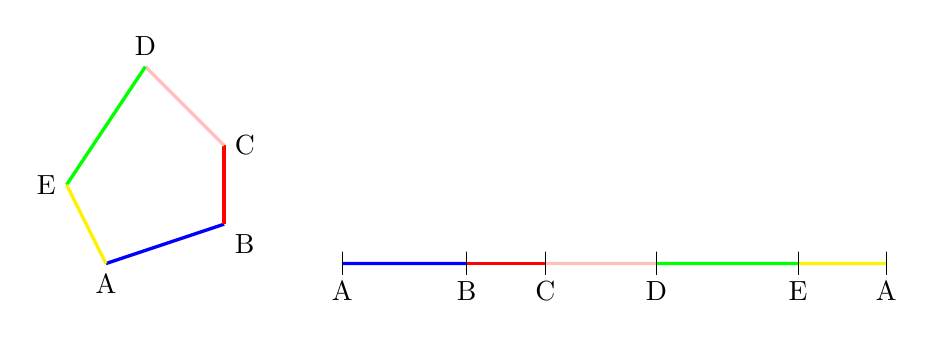
\begin{tikzpicture} % pentagone avec côtés en couleur
\draw [very thick,color=blue] (0,0) node[color=black,below]{A} -- (1.5,0.5) (3,0)--(4.58,0);
\draw [very thick,color=red] (1.5,0.5) node[color=black,below right]{B} -- (1.5,1.5) (4.58,0)--(5.58,0);
\draw [very thick,color=pink] (1.5,1.5) node[color=black,right]{C} -- (0.5,2.5) (5.58,0)--(6.99,0);
\draw [very thick,color=green] (0.5,2.5) node [color=black,above]{D} -- (-0.5,1) (6.99,0)--(8.79,0);
\draw [very thick,color=yellow] (-0.5,1) node[color=black,left]{E} -- (0,0) (8.79,0)--(9.91,0);

\foreach \x / \y in {3/A,4.58/B,5.58/C,6.99/D,8.79/E,9.91/A}
    {\draw (\x,0) node[below=3pt]{\y} --+(0,0.15)--+(0,-0.15);}


\end{tikzpicture} 
\end{center}
Pour exprimer les longueurs, on utilise habituellement pour unité le \textbf{\textcolor{H1}{mètre}} et ses dérivés:
\begin{center}
    \begin{tabular}{|c|c|c|c|c|c|c|}
     \hline   km & hm & dam & m & dm & cm & mm \\ \hline
         & & & & & & \\
    \hline
    \end{tabular}
\end{center}
\end{aconnaitre}

\begin{methode*1}[Transformer des unités de longueurs]

\begin{exemple*1}
Transforme $0,5$ km en m.

Les m (mètres) sont l'unité de mesure.

$1$ km = $\numprint{1000}$ m, donc $0,5$ km $= 0,5 \cdot \numprint{1000}$ m = $500$ m
\end{exemple*1}

\exercice 
Effectue les conversions d'unités de longueur suivantes :
\begin{colenumerate}{3}
 \item $50$ cm en m ;
 \item $100$ mm en m ;
 \item $2,3$ hm en m ;
 \item $0,03$ dm en m ;
 \item $23$ dam en cm ;
 \item $4$ cm en hm.
 \end{colenumerate}
%\correction

\end{methode*1}
%%%%%%%%%%%%%%%%%%%%%%%%%%%%%%%%%%%%%%%%%%%%%%%%%%%%%%%

\section{Aire d'une figure géométrique} 

% remarque : pour qu'un mot se retrouve dans le lexique : \MotDefinition{asymptote horizontale}{} 

\begin{aconnaitre}[Notion de surface]
L' \MotDefinition{aire}{} désigne la valeur de \textbf{\textcolor{H1}{la surface}} occupée par une figure.\\
%le carré
\begin{center}
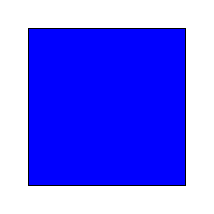
\begin{tikzpicture}
   \begin{scope}[xshift=3cm]
\draw[fill=blue] (0,0)--(2,0) --(2,2) --(0,2) -- cycle;
\end{scope}
\end{tikzpicture}
\end{center}

\prof{
Vous trouverez ici deux lien expliquant le développement du cube et permettant d'expliquer la surface du cube...\\
\href{https://www.geogebra.org/m/arvQstAW}{cube animé}\\
\href{https://www.geogebra.org/m/mZA5qKG9}{patron de cube}
}
Pour exprimer des aires, on utilise habituellement pour unité le \textbf{\textcolor{H1}{mètre carré}} et ses dérivés:
\begin{center}
    \begin{tabular}{|c|c|c|c|c|c|c|c|c|c|c|c|c|c|}
     \hline
     \multicolumn{2}{|c|}{$km^2$} & 
     \multicolumn{2}{c|}{$hm^2$} &
     \multicolumn{2}{c|}{$dam^2$} & 
     \multicolumn{2}{c|}{$m^2$} & 
     \multicolumn{2}{c|}{$dm^2$}  & 
     \multicolumn{2}{c|}{$cm^2$}  & 
     \multicolumn{2}{c|}{$mm^2$}  \\
     \multicolumn{2}{|c|}{} & 
     \multicolumn{2}{c|}{ha} &
     \multicolumn{2}{c|}{a} & 
     \multicolumn{2}{c|}{} & 
     \multicolumn{2}{c|}{}  & 
     \multicolumn{2}{c|}{}  & 
     \multicolumn{2}{c|}{}  \\ \hline
         & & & & & & & & & & & & & \\
    \hline
    \end{tabular}
\end{center}
\end{aconnaitre}

\begin{methode*1}[Pourquoi le tableau des aires comporte des doubles colonnes?]
\begin{exemple*1}\\
Prenons un longueur de 1$cm$.
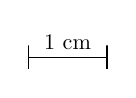
\begin{tikzpicture} %segment de 1cm
\draw (0,0)--(1,0) node[scale=0.8,midway,above]{1 cm};
\draw (0,0)--+(0,0.15)--+(0,-0.15);
\draw (1,0)--+(0,0.15)--+(0,-0.15);
\end{tikzpicture}

Formons une surface basée sur sur cette longueur:
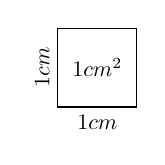
\begin{tikzpicture}%carré de 1cm^2
\draw (0,0)--(1,0) node[scale=0.8,midway,below]{$1 \text{cm}$} --(1,1) --(0,1) -- cycle;
\node[scale=0.8,rotate=90] at(-0.2,0.5) {$1 \text{cm}$};
\node[scale=0.8] at (0.5,0.5) {$1 \text{cm}^2$};
\end{tikzpicture}

L'aire de cette figure est de 1$cm^2$. \\

Maintenant, prenons une longueur dix fois plus grande c'est à dire 10$cm$ soit 1$dm$.\\
\begin{tikzpicture} %segment de 10cm
\draw (0,0)--(10,0) node[scale=0.8,midway,above]{10 cm} node[scale=0.8,midway,below]{1 dm};
\draw (0,0)--+(0,0.15)--+(0,-0.15);
\draw (10,0)--+(0,0.15)--+(0,-0.15);
\end{tikzpicture}

Formons une surface basée sur cette longueur:\\
\begin{tikzpicture}%carré de 100cm^2
\draw (0,0)--(10,0) node[scale=0.8,midway,below]{$10 \text{cm}$} --(10,10) --(0,10) -- cycle;
\node[scale=0.8,rotate=90] at(-0.2,5) {$10 \text{cm}$};
\node[scale=0.8] at (5,5) {$100 \text{cm}^2=1\text{dm}^2$};
\end{tikzpicture}

L'aire est alors de 100$cm^2$.\\
Que remarque-t-on?\\
Lorsqu'une longueur est multipliée par 10, l'aire qui lui est relative est multipliée par 100.\\
La double colonne dans le tableau des aires permet de retranscrire ce phénomène.
\end{exemple*1}
\exercice
Effectue les conversions d'unités d'aire suivantes:
\begin{colenumerate}{3}
 \item $7$ dm\up{2} en m\up{2} ;
 \item $200$ cm\up{2} en m\up{2} ;
 \item $3,2$ ha en m\up{2} ;
 \item $0,8$ dm\up{2} en m\up{2} ;
 \item $45$ hm\up{2} en dm\up{2} ;
 \item $400$ cm\up{2} en a.
 \end{colenumerate}
\end{methode*1}



\begin{methode*1}[Évaluer une aire]
\begin{exemple*1}
\begin{minipage}[c]{0.55\textwidth}
 À l'aide du quadrillage, détermine un encadrement de l'aire de la surface jaune, en prenant pour unité un carreau bleu.
 \end{minipage} \hfill%
 \begin{minipage}[c]{0.2\textwidth}
 \includegraphics[width=2.3cm]{aire1}
 \end{minipage} \\
 
 \begin{minipage}[c]{0.1\textwidth}
  \includegraphics[width=2.3cm]{aire2}
 \end{minipage} \hfill%
 \begin{minipage}[c]{0.7\textwidth}
La surface délimitée en \textbf{\textcolor{H1}{vert}} a une aire plus grande que celle délimitée par la courbe rouge. On compte le nombre de carreaux. Son aire est 18 carreaux.
 \end{minipage} \\[1em]
La surface délimitée en \textbf{noir} a une aire plus petite que celle délimitée par la courbe rouge. On compte le nombre de carreaux. Son aire est quatre carreaux.

Donc l'aire de la figure jaune est comprise entre 4 et 18 carreaux.

\end{exemple*1}

\exercice 
\begin{minipage}[c]{0.50\textwidth}
 Détermine l'aire, en nombre de carrés, des deux figures ci-contre.
 \end{minipage} \hfill%
 \begin{minipage}[c]{0.16\textwidth}
 \includegraphics[width=2.2cm]{aire3}
 \end{minipage} \\
%\correction
 
\end{methode*1}

%%%%%%%%%%%%%%%%%%%%%%%%%%%%%%%%%%%%%%%%%%%%%%%%%%%%%%%

\prof{
\begin{activite}[Problème à Dudu: peindre le cabanon]
\begin{partie}[objectif]
A ce stade, les élèves ne connaissent pas encore les formules de calcul d'aire. Le but est de leur faire découvrir par nécessité. Pour ce faire, ils peuvent avoir accès à différentes ressources bien que tout soit dans le livre.
\end{partie}
\begin{partie}[Mise en place]
Mettre les élèves par groupe de 4 environ.
\end{partie}

\begin{partie}[Consigne]
"on va regarder une vidéo. Tout est indiqué dans le film. Vous allez travailler ensemble pour essayer de répondre à la question qui va vous être posée". Chaque groupe devra rendre son travail qui explique clairement sa démarche sur une feuille A3 (et éventuellement la présenter à la classe!).\\
\end{partie}

\begin{partie}[La vidéo]
Voici le lien qui mène vers la vidéo:
\href{https://www.youtube.com/watch?v=ALUiqD4blG8}{Peindre le cabanon}.
On peut diffuser la vidéo à plusieurs reprises si nécessaire mais il est important que les élèves finissent par prendre des notes.
\end{partie}

\begin{partie}[Déroulement]
Après avoir regardé la vidéo 2 ou 3 fois, les élèves se mettent au travail.\\
Très vite, ils vont avoir besoin de formules qu'ils ne connaissent pas nécessairement. On peut alors les orienter vers les pages du livre correspondantes ou imaginer un prolongement à l'activité avec une tablette ou des ressources mises à disposition dans la classe.\\

Quand les élèves ont terminé, on peut imaginer une rapide présentation de leur travail à la classe. On peut afficher les travaux ou les noter...\\

Voici le genre de travail attendu....:
\begin{center}
\includegraphics[width=14cm]{PerimetresAires/figures/cabanon.eps} 
\end{center}

\end{partie}
\end{activite}
}

%%%%%%%%%%%%%%%%%%%%%%%%%%%%%%%%%%%%%%%%%%%%%%%%%%%%%%%

\section{Volume d'un solide}

\begin{aconnaitre}[Notion de volume]
Le mot \MotDefinition{volume}{} désigne l'espace contenu dans une figure en 3 dimensions.\\
Pour exprimer des volumes, on utilise habituellement pour unité le \textbf{\textcolor{H1}{mètre cube}} et ses dérivés:
\begin{center}
    \begin{tabular}{|c|c|c|c|c|c|c|c|c|c|c|c|c|c|c|c|c|c|c|c|c|}
     \hline
     \multicolumn{3}{|c|}{$km^3$} & 
     \multicolumn{3}{c|}{$hm^3$} &
     \multicolumn{3}{c|}{$dam^3$} & 
     \multicolumn{3}{c|}{$m^3$} & 
     \multicolumn{3}{c|}{$dm^3$}  & 
     \multicolumn{3}{c|}{$cm^3$}  & 
     \multicolumn{3}{c|}{$mm^3$}  \\    \hline
         & & & & & & & & & & & & & & & & & & & & \\
    \hline
    \end{tabular}
\end{center}
\end{aconnaitre}

\begin{methode*1}[Pourquoi le tableau des volumes comporte des triples colonnes?]
\begin{exemple*1}\\
On a vu précédemment que lorsque la longueur d'un carré est multipliée par 10, son aire est multipliée par 100.\\
Il en va de même avec les volumes. Lorsque la longueur d'un cube est multipliée par 10, le volume se trouve multiplié par 1000. C'est pour retranscrire ce phénomène que le tableau des volumes comporte des triples colonnes.
\end{exemple*1}
\exercice
Effectue les conversions d'unités de volume suivantes:
\begin{colenumerate}{3}
 \item $7,61$ km\up{3} en hm\up{3} ;
 \item $5,15$ m\up{3} en cm\up{3} ;
 \item $8,12$ cm\up{3}  en dm\up{3} ;
 \item $12,1$ m\up{3} en hm\up{3} ;
 \item $85,3$ hm\up{3} en dam\up{3} ;
 \item $48,7$ dam\up{3} en m\up{3}.
 \end{colenumerate}
\end{methode*1}


%%%%%%%%%%%%%%%%%%%%%%%%%%%%%%%%%%%%%%%%%%%%%%%%%%%%%%%%%%%%%%%%%
\begin{center}
    \textsc{\textbf{POUR RÉSUMER...}}\\
    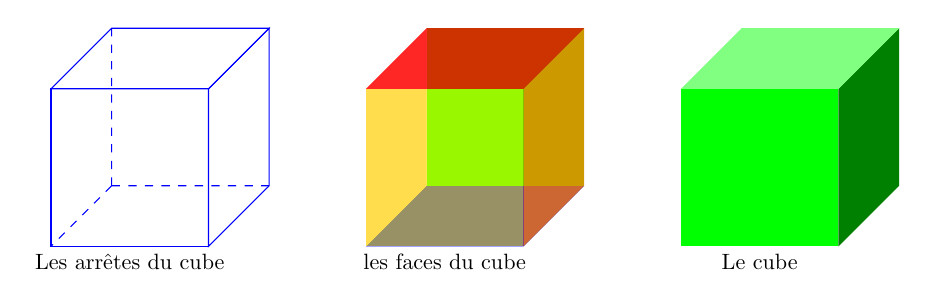
\begin{tikzpicture} 
\def \Width {2};
\def \Height {2};
\def \Depth {2};

%les arrêtes du cube
\begin{scope}
\def \translate {0};
\coordinate (O) at (0+\translate,0,0);
\coordinate (A) at (0+\translate,\Width,0);
\coordinate (B) at (0+\translate,\Width,\Height);
\coordinate (C) at (0+\translate,0,\Height);
\coordinate (D) at (\Depth+\translate,0,0);
\coordinate (E) at (\Depth+\translate,\Width,0);
\coordinate (F) at (\Depth+\translate,\Width,\Height);
\coordinate (G) at (\Depth+\translate,0,\Height);

\draw[dashed, blue] (O) -- (A) (O) -- (C) (O) -- (D);% arrêtes cachées
\draw[blue] (D) -- (E) -- (F) -- (G) -- cycle;% Right Face
\draw[blue] (C) -- (B) -- (F) -- (G) -- cycle;% Front Face
\draw[blue] (A) -- (B) -- (F) -- (E) -- cycle;% Top Face

\path (C)--(G) node[scale=0.8,midway,below]{Les arrêtes du cube};

%\node at (A) {A};
%\node at (B) {B};
%\node at (C) {C};
%\node at (D) {D};
%\node at (E) {E};
%\node at (F) {F};
%\node at (G) {G};
\end{scope}

%les faces du cubes
\begin{scope}
\def \translate {4};

\coordinate (O) at (0+\translate,0,0);
\coordinate (A) at (0+\translate,\Width,0);
\coordinate (B) at (0+\translate,\Width,\Height);
\coordinate (C) at (0+\translate,0,\Height);
\coordinate (D) at (\Depth+\translate,0,0);
\coordinate (E) at (\Depth+\translate,\Width,0);
\coordinate (F) at (\Depth+\translate,\Width,\Height);
\coordinate (G) at (\Depth+\translate,0,\Height);

\fill[blue] (O) -- (C) -- (G) -- (D) -- cycle;% Bottom Face
\fill[green] (O) -- (A) -- (E) -- (D) -- cycle;% Back Face
\fill[pink] (O) -- (A) -- (B) -- (C) -- cycle;% Left Face
\fill[orange,opacity=0.8] (D) -- (E) -- (F) -- (G) -- cycle;% Right Face
\fill[yellow,opacity=0.6] (C) -- (B) -- (F) -- (G) -- cycle;% Front Face
\fill[red,opacity=0.8] (A) -- (B) -- (F) -- (E) -- cycle;% Top Face


\path (C)--(G) node[scale=0.8,midway,below]{les faces du cube};
%\path (A)--(E) node[scale=0.8,midway,above]{solide (ou volume?)};

%\node at (A) {A};
%\node at (B) {B};
%\node at (C) {C};
%\node at (D) {D};
%\node at (E) {E};
%\node at (F) {F};
%\node at (G) {G};
\end{scope}

%le cube
\begin{scope}
\def \translate {8};

\coordinate (O) at (0+\translate,0,0);
\coordinate (A) at (0+\translate,\Width,0);
\coordinate (B) at (0+\translate,\Width,\Height);
\coordinate (C) at (0+\translate,0,\Height);
\coordinate (D) at (\Depth+\translate,0,0);
\coordinate (E) at (\Depth+\translate,\Width,0);
\coordinate (F) at (\Depth+\translate,\Width,\Height);
\coordinate (G) at (\Depth+\translate,0,\Height);

%\draw (O) -- (C) -- (G) -- (D) -- cycle;% Bottom Face
%\draw (O) -- (A) -- (E) -- (D) -- cycle;% Back Face
%\draw (O) -- (A) -- (B) -- (C) -- cycle;% Left Face
\fill[green!50!black] (D) -- (E) -- (F) -- (G) -- cycle;% Right Face
\fill[green] (C) -- (B) -- (F) -- (G) -- cycle;% Front Face
\fill[green!50!white] (A) -- (B) -- (F) -- (E) -- cycle;% Top Face


\path (C)--(G) node[scale=0.8,midway,below]{Le cube};
%\path (A)--(E) node[scale=0.8,midway,above]{solide (ou volume?)};

%\node at (A) {A};
%\node at (B) {B};
%\node at (C) {C};
%\node at (D) {D};
%\node at (E) {E};
%\node at (F) {F};
%\node at (G) {G};
\end{scope}


\end{tikzpicture}

\end{center}

%%%%%%%%%%%%%%%%%%%%%%%%%%%%%%%%%%%%%%%%%%%%%%%%%%%%%%%%%%%%%%%%%

\newpage

\vspace{2em}
\section{Calculer des aires à l'aide d'une formule}

\begin{aconnaitre}[aire du rectangle et du triangle rectangle]
\begin{tabularx}{\linewidth}{|c|X|X|}
 \cline{2-3}
\multicolumn{1}{c|}{} & \begin{center} \textbf{\textcolor{H1}{Rectangle}} \includegraphics[width=2.5cm]{rectangleLI} \end{center} & \begin{center} \textbf{\textcolor{H1}{Triangle rectangle}} \includegraphics[width=2.7cm]{rectangleABCD4} \end{center} \\ \hline
Formule & L'aire du rectangle peut se calculer avec cette formule : {\large \textbf{$\mathcal{A} = L \cdot \ell$}} & L'aire de $ABD$ est égale à la moitié de l'aire de $ABCD$ : {\large \textbf{$\mathcal{A} = \dfrac{AB \cdot AD}{2}$}} \phantom{retourligne} \\\hline
 \end{tabularx} \\[1em]
Les longueurs doivent être exprimées dans la même unité.
\end{aconnaitre}
\begin{methode*1}
\begin{exemple*1}
Calcule l'aire de la figure $ABCDE$ ci‑dessous (L'unité de longueur est le centimètre) :
\begin{center}  \includegraphics[width=4.3cm]{aire4} \end{center}

 \begin{itemize}
  \item La figure est composée du rectangle $ABDE$ et du triangle rectangle $BCD$. Son aire est donc égale à la somme de l'aire de $ABDE$ et de l'aire de $BCD$ ;
  \item $\mathcal{A}_{ABDE} = AB \cdot AE = 7$ cm $\cdot$ $2,5$ cm = $17,5$ cm\up{2} ; \\[0.2em]
  \item $\mathcal{A}_{BCD} = \dfrac{BC \cdot BD}{2} = \dfrac{5,4 \text{ cm} \cdot 2,5 \text{ cm}}{2} = \dfrac{13,5 \text{ cm}\up{2}}{2} = 6,75 $ cm\up{2} ;\\[0.2em]
  \item $\mathcal{A}_{ABCDE} = 17,5$ cm\up{2} $+ 6,75$ cm\up{2} = $24,25$ cm\up{2}.
  \item L'aire de la figure $ABCDE$ est donc égale à $24,25$ cm\up{2}.
  \end{itemize}
\end{exemple*1}

\exercice 
Détermine l'aire d'un carré de côté 6 cm. 
%\correction

\exercice 
Détermine l'aire d'un rectangle de longueur 3 cm et de largeur 22 mm en donnant le résultat en cm\up{2}.
%\correction
     
\exercice 
$SON$ est un triangle rectangle en $S$, tel que 

$SO = 8,04$ dm et $SN = 0,93$ m. Détermine son aire en donnant le résultat en m\up{2}.
%\correction
 
\end{methode*1}
%%%%%%%%%%%%%%%%%%%%%%%%%%%%%%%%%%%%%%%%%%%%%%%%%%%%%%%%
\newpage

\vspace{2em}

\begin{aconnaitre}[Aire d'un triangle]
Pour calculer l’aire d’un triangle, on multiplie la \textbf{\textcolor{H1}{longueur d'un côté}} par la \textbf{\textcolor{C2}{hauteur}} relative à ce côté puis on divise le résultat par 2 :

\begin{tabularx}{\textwidth}{XX}
{\large $\mathcal{A} = \dfrac{b \cdot h}{2}$} & \includegraphics[width=5cm]{longueur_hauteur} \\
 \end{tabularx} \\
 \end{aconnaitre}

\vspace{4em}

\begin{methode*1}[Calculer l’aire d’un triangle]


 
\begin{exemple*1}
Calcule l’aire du triangle suivant :
\begin{minipage}[c]{0.68\textwidth}
\begin{itemize}
 \item On mesure la longueur d'un côté ;
 \item On mesure la hauteur relative à ce côté ;
 \item On multiplie la longueur du côté repéré par la hauteur relative à ce côté puis on divise le résultat par 2 : \\[0.3em]
$\mathcal{A} = \dfrac{10 \cdot 3}{2} = \dfrac{30}{2} = 15$. \\[0.3em]
L'aire du triangle vaut 15 cm\up{2}.
 \end{itemize}
 \end{minipage} \hfill%
 \begin{minipage}[c]{0.2\textwidth}
 \includegraphics[width=3.5cm]{triangle_croquisZ}
 \end{minipage} \\
\end{exemple*1}


\exercice 
Calcule l’aire des triangles suivants :
\begin{colenumerate}{2}
 \item
 
 \includegraphics[width=3.1cm]{triangle_croquisY}
 \item
 
 \includegraphics[width=2.8cm]{triangle_croquisW}
 \end{colenumerate}
%\correction

\end{methode*1}
%%%%%%%%%%%%%%%%%%%%%%%%%%%%%%%%%%%%%%%%%%%%%%%%%%%%%%%%
\newpage

\vspace{2em}

\begin{aconnaitre}[Aire d'un parallélogramme]
Pour calculer l’\MotDefinition{aire d’un parallélogramme}{}, on multiplie la \textbf{\textcolor{H1}{longueur d'un côté}} par la \textbf{\textcolor{C2}{hauteur}} relative à ce côté :

\vspace{1em}

\begin{tabularx}{\textwidth}{XX}
{\large $\mathcal{A} = b \cdot h$} & \includegraphics[width=4cm]{parallelogrammehb} \\
 \end{tabularx} \\

\end{aconnaitre}


\vspace{4em}

\begin{methode*1}[Calculer l’aire d’un parallélogramme]


\begin{exemple*1}
Détermine l’\textbf{aire} du parallélogramme suivant :
\begin{minipage}[c]{0.65\textwidth}
\begin{itemize}
 \item On mesure la \textbf{\textcolor{H1}{longueur}} d'un côté ;
 \item On mesure la \textbf{\textcolor{C2}{hauteur}} relative à ce côté ;
 \item On multiplie la longueur du côté repéré par la hauteur relative à ce côté : $\mathcal{A} = 12 \cdot 5 = 60$ ;
 \item L'aire du parallélogramme vaut 60 cm\up{2}.
 \end{itemize}
 \end{minipage} \hfill%
 \begin{minipage}[c]{0.26\textwidth}
 \includegraphics[width=3cm]{parallelog_croquis}
 \end{minipage} \\
\end{exemple*1}

\exercice 
Détermine l’aire des parallélogrammes $MNOP$ et $ABCD$ ci-dessous :
\begin{colenumerate}{2}
 \item 
 
 \includegraphics[width=3.7cm]{parallelogMNPO}
 \item 
 
 \includegraphics[width=4.4cm]{parallelogABCD}
 \end{colenumerate}
%\correction

\end{methode*1}
%%%%%%%%%%%%%%%%%%%%%%%%%%%%%%%%%%%%%%%%%%%%%%%%%%%%%%%%



\newpage

\vspace{2em}

\begin{aconnaitre}[Aire d'un losange]
Pour calculer l’aire d’un losange, on effectue le produit des \textbf{\textcolor{H1}{longueurs des diagonales}} puis on divise le résultat par 2 : 

\begin{tabularx}{\textwidth}{XX}
{\large $\mathcal{A} = \dfrac{d \cdot D}{2}$} & \includegraphics[width=5cm]{losangeDd} \\
 \end{tabularx} \\
 \end{aconnaitre}

\vspace{4em}

\begin{methode*1}[Calculer l’aire d’un losange]


 
 \begin{exemple*1}
Calcule l’aire du losange suivant :
\begin{minipage}[c]{0.68\textwidth}
\begin{itemize}
 \item On repère la longueur des diagonales.
 \item On calcule le produit des longueurs des diagonales puis on divise le résultat par 2 : \\[0.3em]
$\mathcal{A} = \dfrac{10 \cdot 5}{2} = \dfrac{50}{2} = 25$ \\[0.3em]
L'aire du losange vaut 25 cm\up{2}.
 \end{itemize}
 \end{minipage} \hfill%
 \begin{minipage}[c]{0.2\textwidth}
 \includegraphics[width=2.9cm]{losange26}
 \end{minipage} \\
\end{exemple*1}

 
 \exercice
Calcule l’aire des losanges suivants :
\begin{colenumerate}{2}
 \item
 
 \includegraphics[width=5cm]{losange12_10}
 \item
 
 \includegraphics[width=4cm]{losange10_10}
 \end{colenumerate}
%\correction

\end{methode*1}



\exercicesbase
\begin{colonne*exercice}
\input{PerimetresAires/PerimetresAires_exos_entrain.tex}
\end{colonne*exercice}


\exercicesappr
\begin{colonne*exercice}
\input{PerimetresAires/PerimetresAires_exos_approf}
\end{colonne*exercice}

\connaissances
\input{PerimetresAires/PerimetresAires_qcm.tex}

\TravauxPratiques % pour nous "travailler en groupe"
\input{PerimetresAires/PerimetresAires_en_groupe.tex}

\pagebreak

\recreation
\begin{enigme}[Invitation au bal]
Sur le carton d'invitation rectangulaire ci-contre, toutes les longueurs sont données en centimètres. Quel est le mot de passe ?
\vspace{1cm}
\begin{center} 
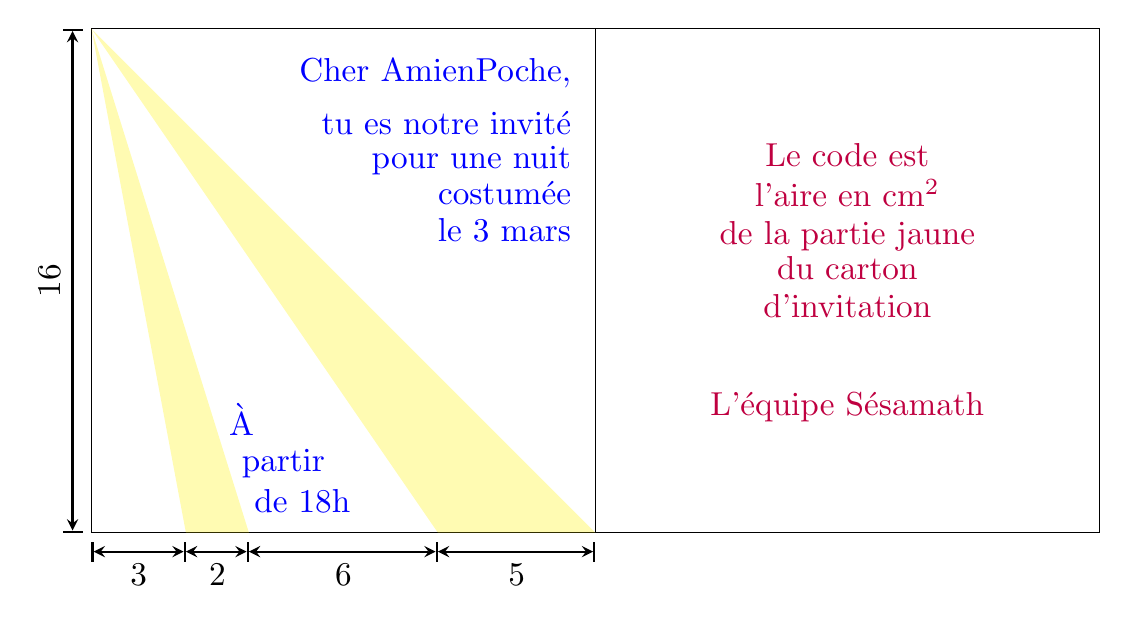
\begin{tikzpicture}[every node/.style={scale=1.2},scale=0.8]
 \draw (0,0)--(0,8)--(16,8)--(16,0)--cycle;
 \draw (8,8)--(8,0);
 \fill [yellow,opacity=0.3] (0,8)--(2.5,0)--(1.5,0)--cycle;
 \fill [yellow,opacity=0.3] (0,8)--(8,0)--(5.5,0)--cycle;
 
\draw (7.8,7.3) node[left,blue] {Cher AmienPoche,};
\draw (7.8,6.5) node[left,blue] {tu es notre invité};
\draw (7.8,5.9) node[left,blue] {pour une nuit};
\draw (7.8,5.4) node[left,blue] {costumée};
\draw (7.8,4.8) node[left,blue] {le 3 mars};

\draw (2,1.8) node[right,blue] {À};
\draw (2.2,1.1) node[right,blue] {partir};
\draw (2.4,0.5) node[right,blue] {de 18h};

\draw (12,6) node[purple] {Le code est};
\draw (12,5.4) node[purple] {l'aire en cm$^2$};
\draw (12,4.7) node[purple] {de la partie jaune};
\draw (12,4.2) node[purple] {du carton};
\draw (12,3.6) node[purple] {d'invitation};
\draw (12,2) node[purple] {L'équipe Sésamath};

\draw [thick,|<->|,>=stealth](-0.3,0)--(-0.3,8) node [midway,above,rotate=90]{16};
\draw [thick,|<->|,>=stealth](0,-0.3)--(1.5,-0.3) node [midway,below]{3};
\draw [thick,<->|,>=stealth](1.5,-0.3)--(2.5,-0.3) node [midway,below]{2};
\draw [thick,<->|,>=stealth](2.5,-0.3)--(5.5,-0.3) node [midway,below]{6};
\draw [thick,<->|,>=stealth](5.5,-0.3)--(8,-0.3) node [midway,below]{5};

\end{tikzpicture}

\end{center}
 
 \end{enigme}
 

 



